\documentclass{article}
\usepackage{geometry}
\usepackage{graphicx}
\usepackage{amsmath}
\usepackage{hyperref}
\usepackage{lipsum}
\usepackage{booktabs}
\geometry{a4paper, margin=1in}

\setlength{\parindent}{0pt}

\begin{document}

\begin{titlepage}
    \begin{center}
        \vspace*{1.5cm}
        
        \Huge
        \textbf{Group Project}
        
        \Large
        \vspace{1.5cm}
        
            \textbf{Laurie Byrne}\\
            \textbf{Harry Fitzgerald}\\
            \textbf{Liam Power}\\
            \textbf{George Levins}\\

        \vspace{1.5cm}
        30th November 2024
        
        \vspace{3cm}
        
        
\includegraphics[width=0.8\textwidth]{Trinity_Main_Logo.jpg}

        \vspace{2cm}
        \vfill
        {\large This document is submitted as part of the coursework for STU22004 Applied Probability}
        
    \end{center}    
\end{titlepage}

\newpage
\section*{Question 1}
Consider a scenario where the temperature \(X(t)\) varies randomly over a continuous time interval \(t\), where \(t\) is in the range from 0 to 1. We begin with the assumption that \(X(0)=0\), which means that the temperature at time 0 is 0. Now, if we choose a small time increment represented by \(\Delta t\), we can make the assumption that the change in temperature from time \(t\) to \(t+\Delta t\), denoted as \(X(t+\Delta t)-X(t)\), follows a normal distribution. This normal distribution is characterized by a mean of 0 and a variance of \(\Delta t\).\\

1. Let \(P\) be the random variable denoting the proportion of time in \([0,1]\) such that the temperature is positive. Estimate the distribution of \(P\) by Monte Carlo simulation and experimenting with various values of \(\Delta t\) (e.g., \(\Delta t=0.01, 0.001, 0.0001, \ldots\)).\\

2. Let \(T_{\max}\) be the random variable denoting the time in \([0,1]\) such that the temperature is at its maximum. Estimate the distribution of \(T_{\max}\) by Monte Carlo simulation and experimenting with various values of \(\Delta t\) (e.g., \(\Delta t=0.01, 0.001, 0.0001, \ldots\)).

\subsection*{Question 1.1}

\subsubsection*{Method}
To calculate the proportion of time that the temperature \(X(t)\) is positive, you can follow a structured approach using Monte Carlo simulations. This involves several key steps that ensure a comprehensive analysis of the temperature changes over a specified time interval.\\

\textbf{Create a Discrete Time Interval:}
Since the temperature \(X(t)\) varies continuously from \(t = 0\) to \(t = 1\), we need to discretize this interval. This means dividing the continuous time into small, manageable steps, each separated by a time increment \(\Delta t\). The total number of steps can be calculated as \(\frac{1}{\Delta t}\).\\

\textbf{Run Simulation of Temperature Change:} \\
The simulation aims to model how the temperature changes over time. Starting with the initial condition \(X(0) = 0\), each subsequent temperature change from one time point to the next is given by \(X(t + \Delta t) - X(t)\). This change follows a normal distribution with a mean of 0 and variance \(\Delta t\). The formula used for simulation is:
\[
X(t_{i+1}) = X(t_i) + Z_i
\]
Here, \(Z_i\) is a random variable drawn from a normal distribution with mean 0 and variance \(\Delta t\), representing the random fluctuation in temperature.\\

\textbf{Calculate the Proportion of Positive Time:} \\
To determine how often the temperature is positive, calculate the proportion \(P\) by dividing the number of positive temperature steps by the total number of steps:
\[
P = \frac{\text{Positive Steps}}{\text{Total Number of Steps}}
\]

\textbf{Repeat Simulation:}
To estimate the distribution of \(P\), repeat the simulation multiple times. Each iteration provides a different value for \(P\), capturing the variability inherent in random processes.\\

\textbf{Analyze Results:}
After running enough simulations, you will have a collection of \(P\) values. Analyze these results by creating histograms and calculating summary statistics to describe their distribution.\\

\textbf{Repeat with Different Values of \(\Delta t\):} \\
To improve accuracy, repeat the entire process with different values of \(\Delta t\), such as 0.01, 0.001, and 0.0001. Smaller values of \(\Delta t\) provide finer granularity and can lead to more accurate approximations.

\subsubsection*{Code}

\begin{verbatim}
    import numpy as np
    import matplotlib.pyplot as pyplot
    
    numberOfSimulations = 10000
    deltaTValue = 100
    
    deltaT = 1 / deltaTValue                                                            
    times = np.zeros((numberOfSimulations, deltaTValue))                                          
    
    for i in range(1, deltaTValue):                                                     
        increments = np.random.normal(0, np.sqrt(deltaT), numberOfSimulations)          
        times[:, i] = times[:, i - 1] + increments
    
    numberOfPositives = np.sum(times > 0, axis = 1)
    proportions = numberOfPositives / deltaTValue
    
    pyplot.figure(figsize=(12, 6))
    pyplot.hist(proportions, bins=30, alpha=0.5, edgecolor='black', label=f'deltaT = 
    {deltaT}')
    pyplot.title('Distribution of Proportion of Positive Temperature Over Time')
    pyplot.xlabel('Proportion of positive temperature')
    pyplot.ylabel('Frequency')
    pyplot.legend(loc='upper right')
    pyplot.show()
\end{verbatim}

\subsubsection*{Figures}

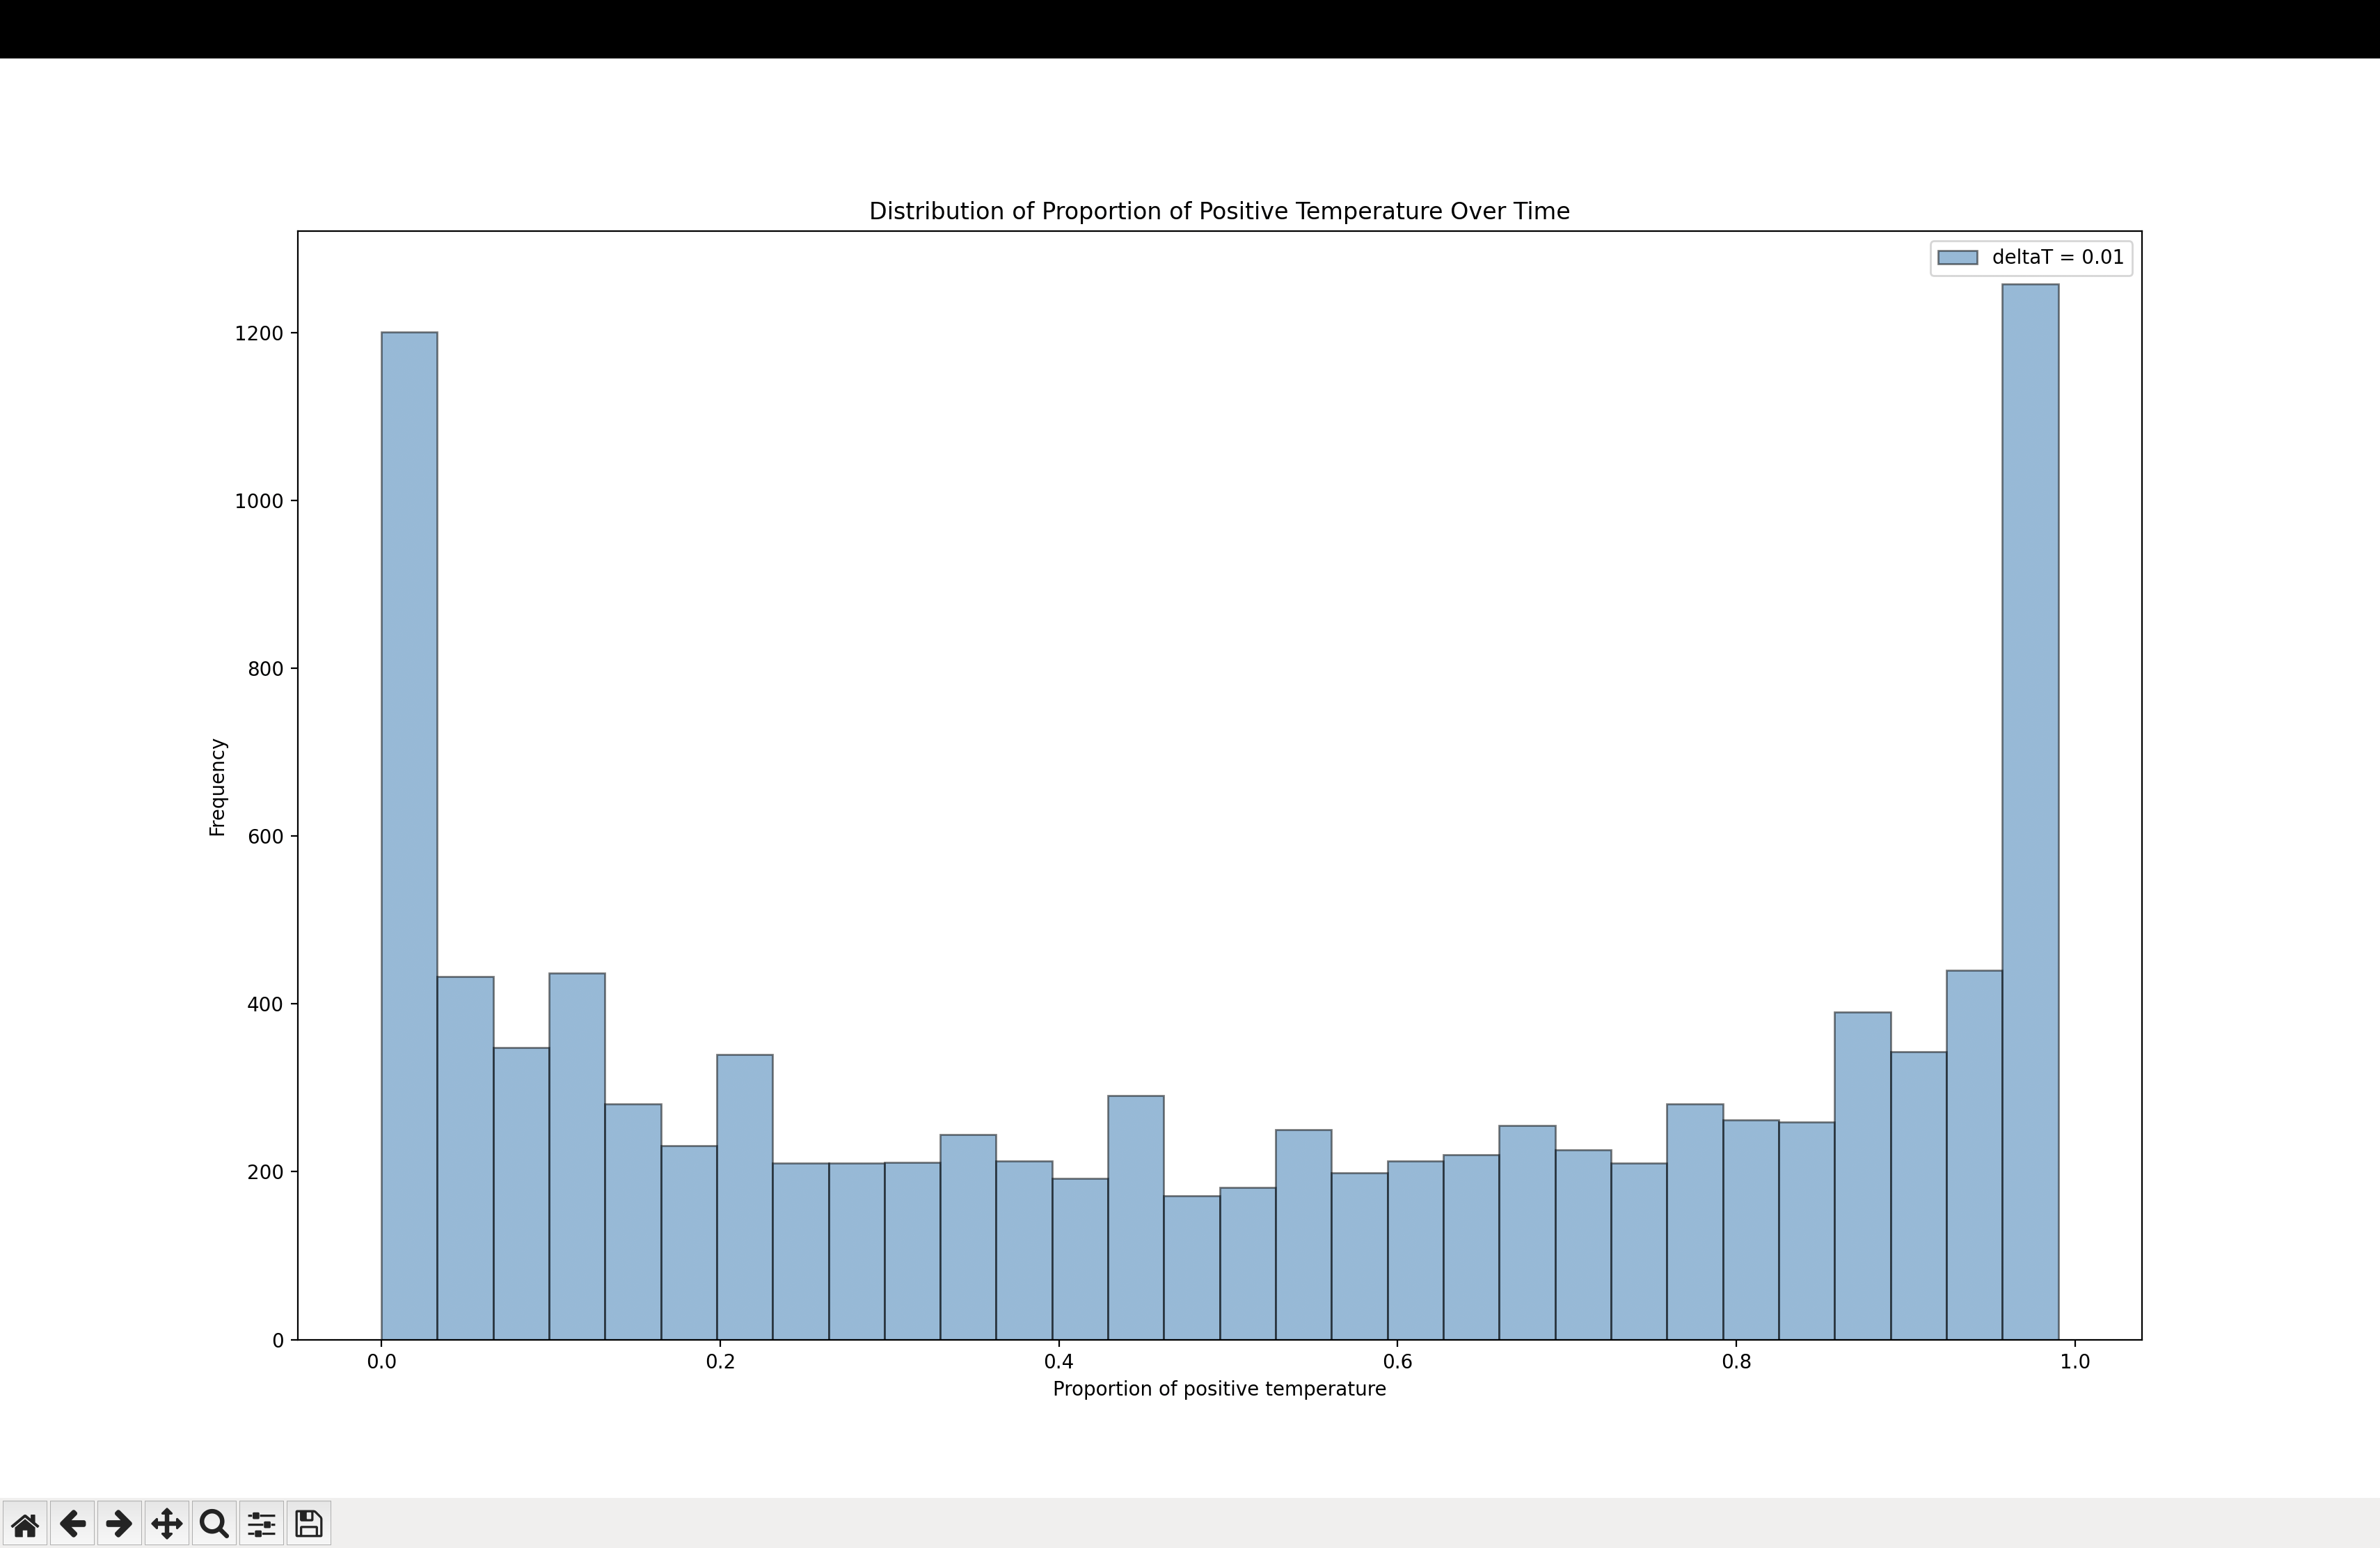
\includegraphics[width=0.6\textwidth]{q1_p1_f1.png}

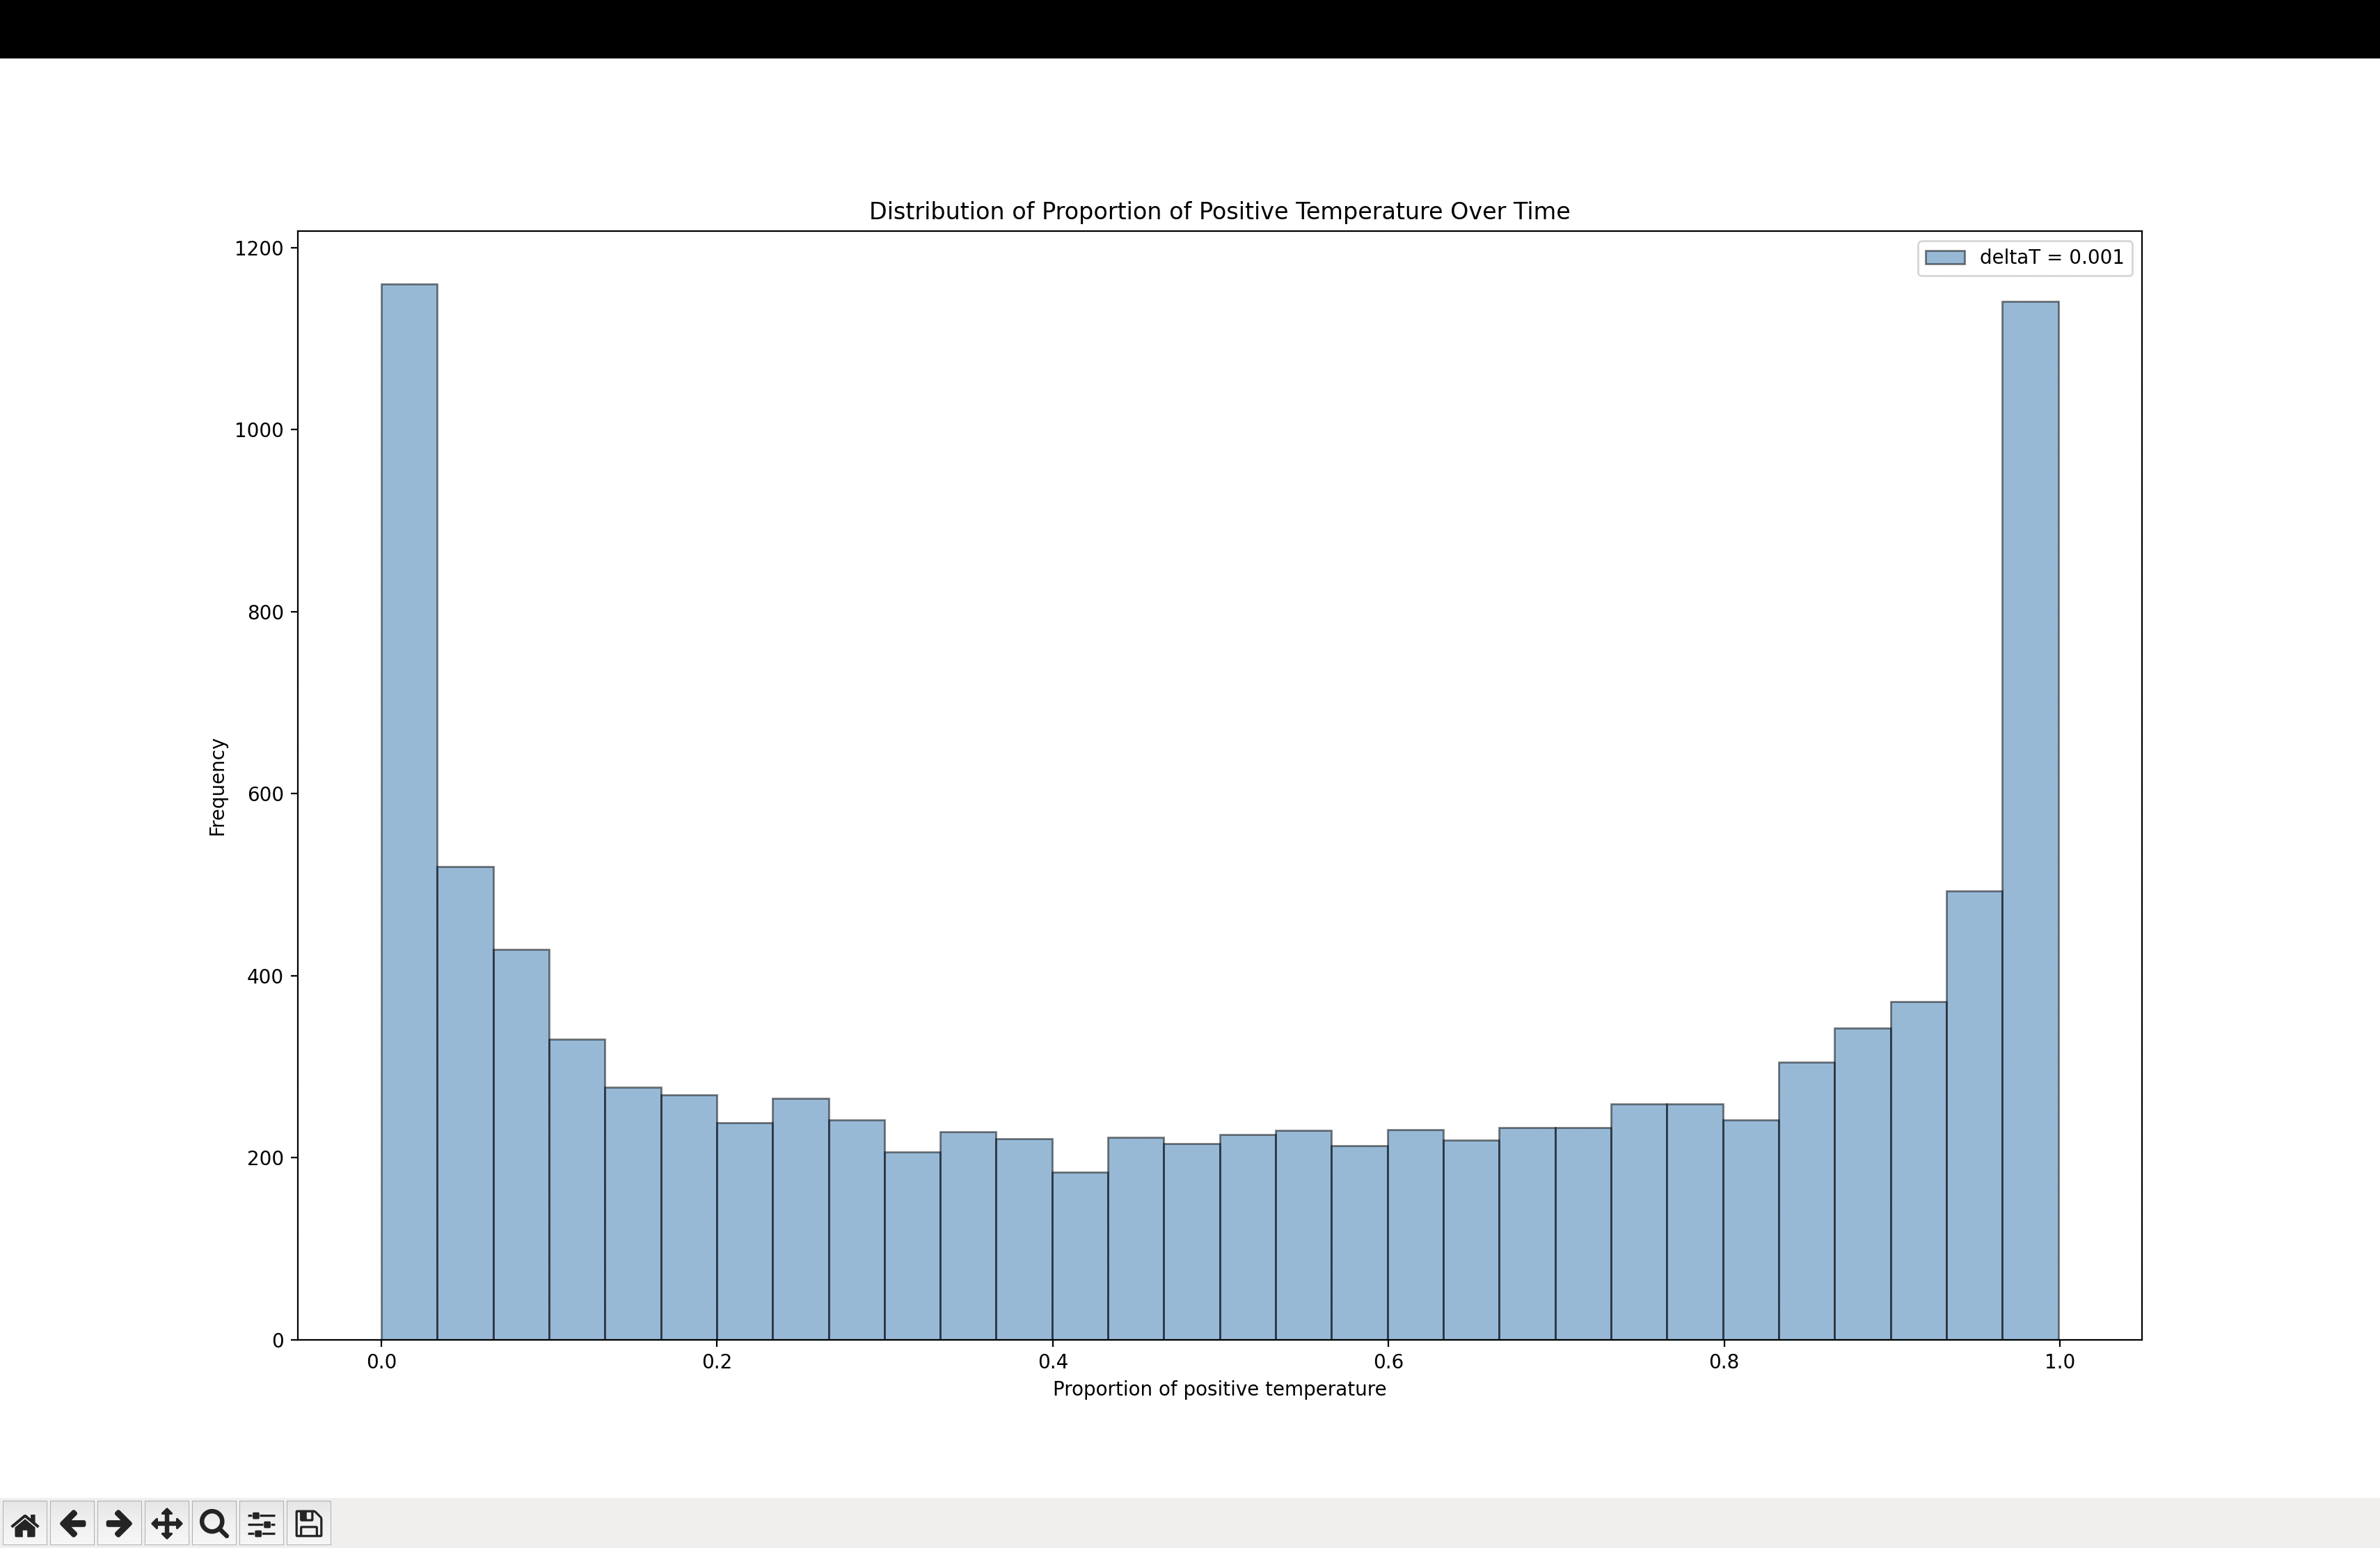
\includegraphics[width=0.6\textwidth]{q1_p1_f2.png}

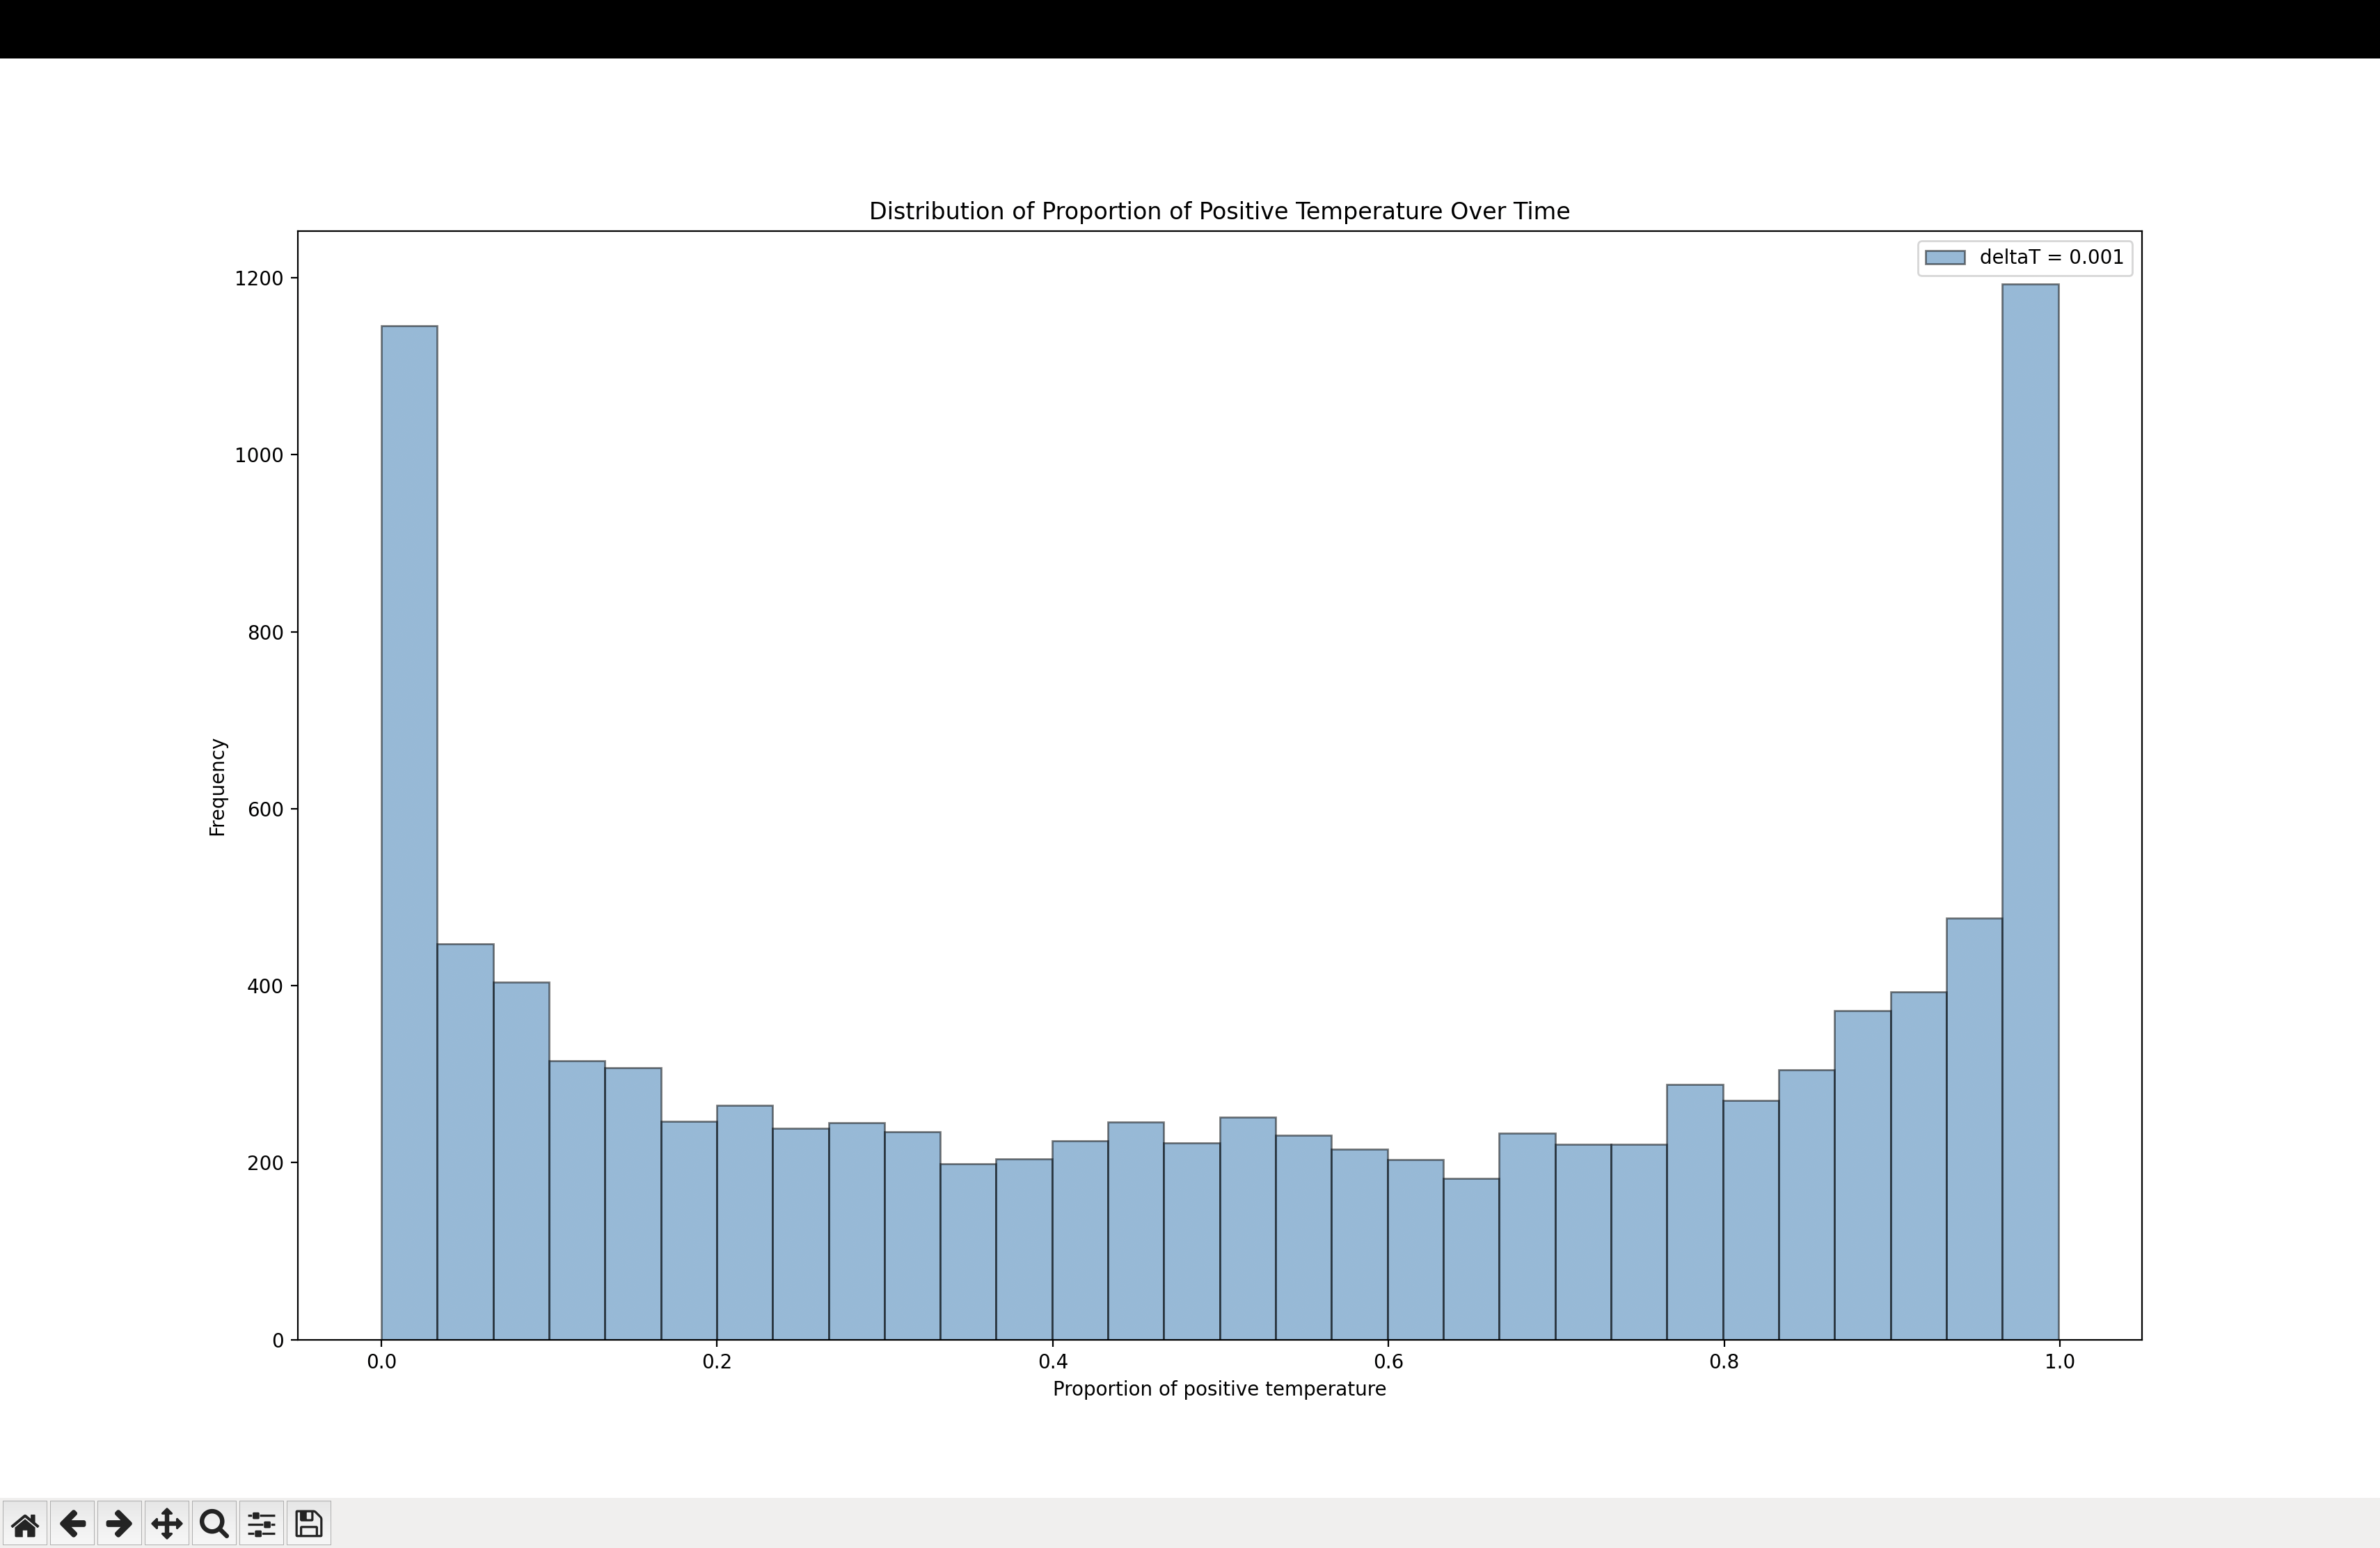
\includegraphics[width=0.6\textwidth]{q1_p1_f3.png}


\subsection*{Question 1.2}

\subsubsection*{Method}
\lipsum[1]\\

\lipsum[2]\\

\subsubsection*{Code}

\begin{verbatim}
    import numpy as np
    import matplotlib.pyplot as pyplot
    
    numberOfSimulations = 10000
    deltaTValue = 10000
    
    deltaT = 1 / deltaTValue                                                            
    times = np.zeros((numberOfSimulations, deltaTValue))                                          
    
    for i in range(1, deltaTValue):                                                     
        increments = np.random.normal(0, np.sqrt(deltaT), numberOfSimulations)          
        times[:, i] = times[:, i - 1] + increments
    
    maxIndices = np.argmax(times, axis=1)
    maxTimes = maxIndices * deltaT
    
    pyplot.hist(maxTimes, bins=30, alpha=0.5, edgecolor='black', label=f'deltaT = 
    {deltaT}')
    pyplot.title('Distribution of Time at Maximum Temperature')
    pyplot.xlabel('Time of maximum temperature')
    pyplot.ylabel('Frequency')
    pyplot.legend(loc='upper right')
    pyplot.show() 
\end{verbatim}

\subsubsection*{Figures}

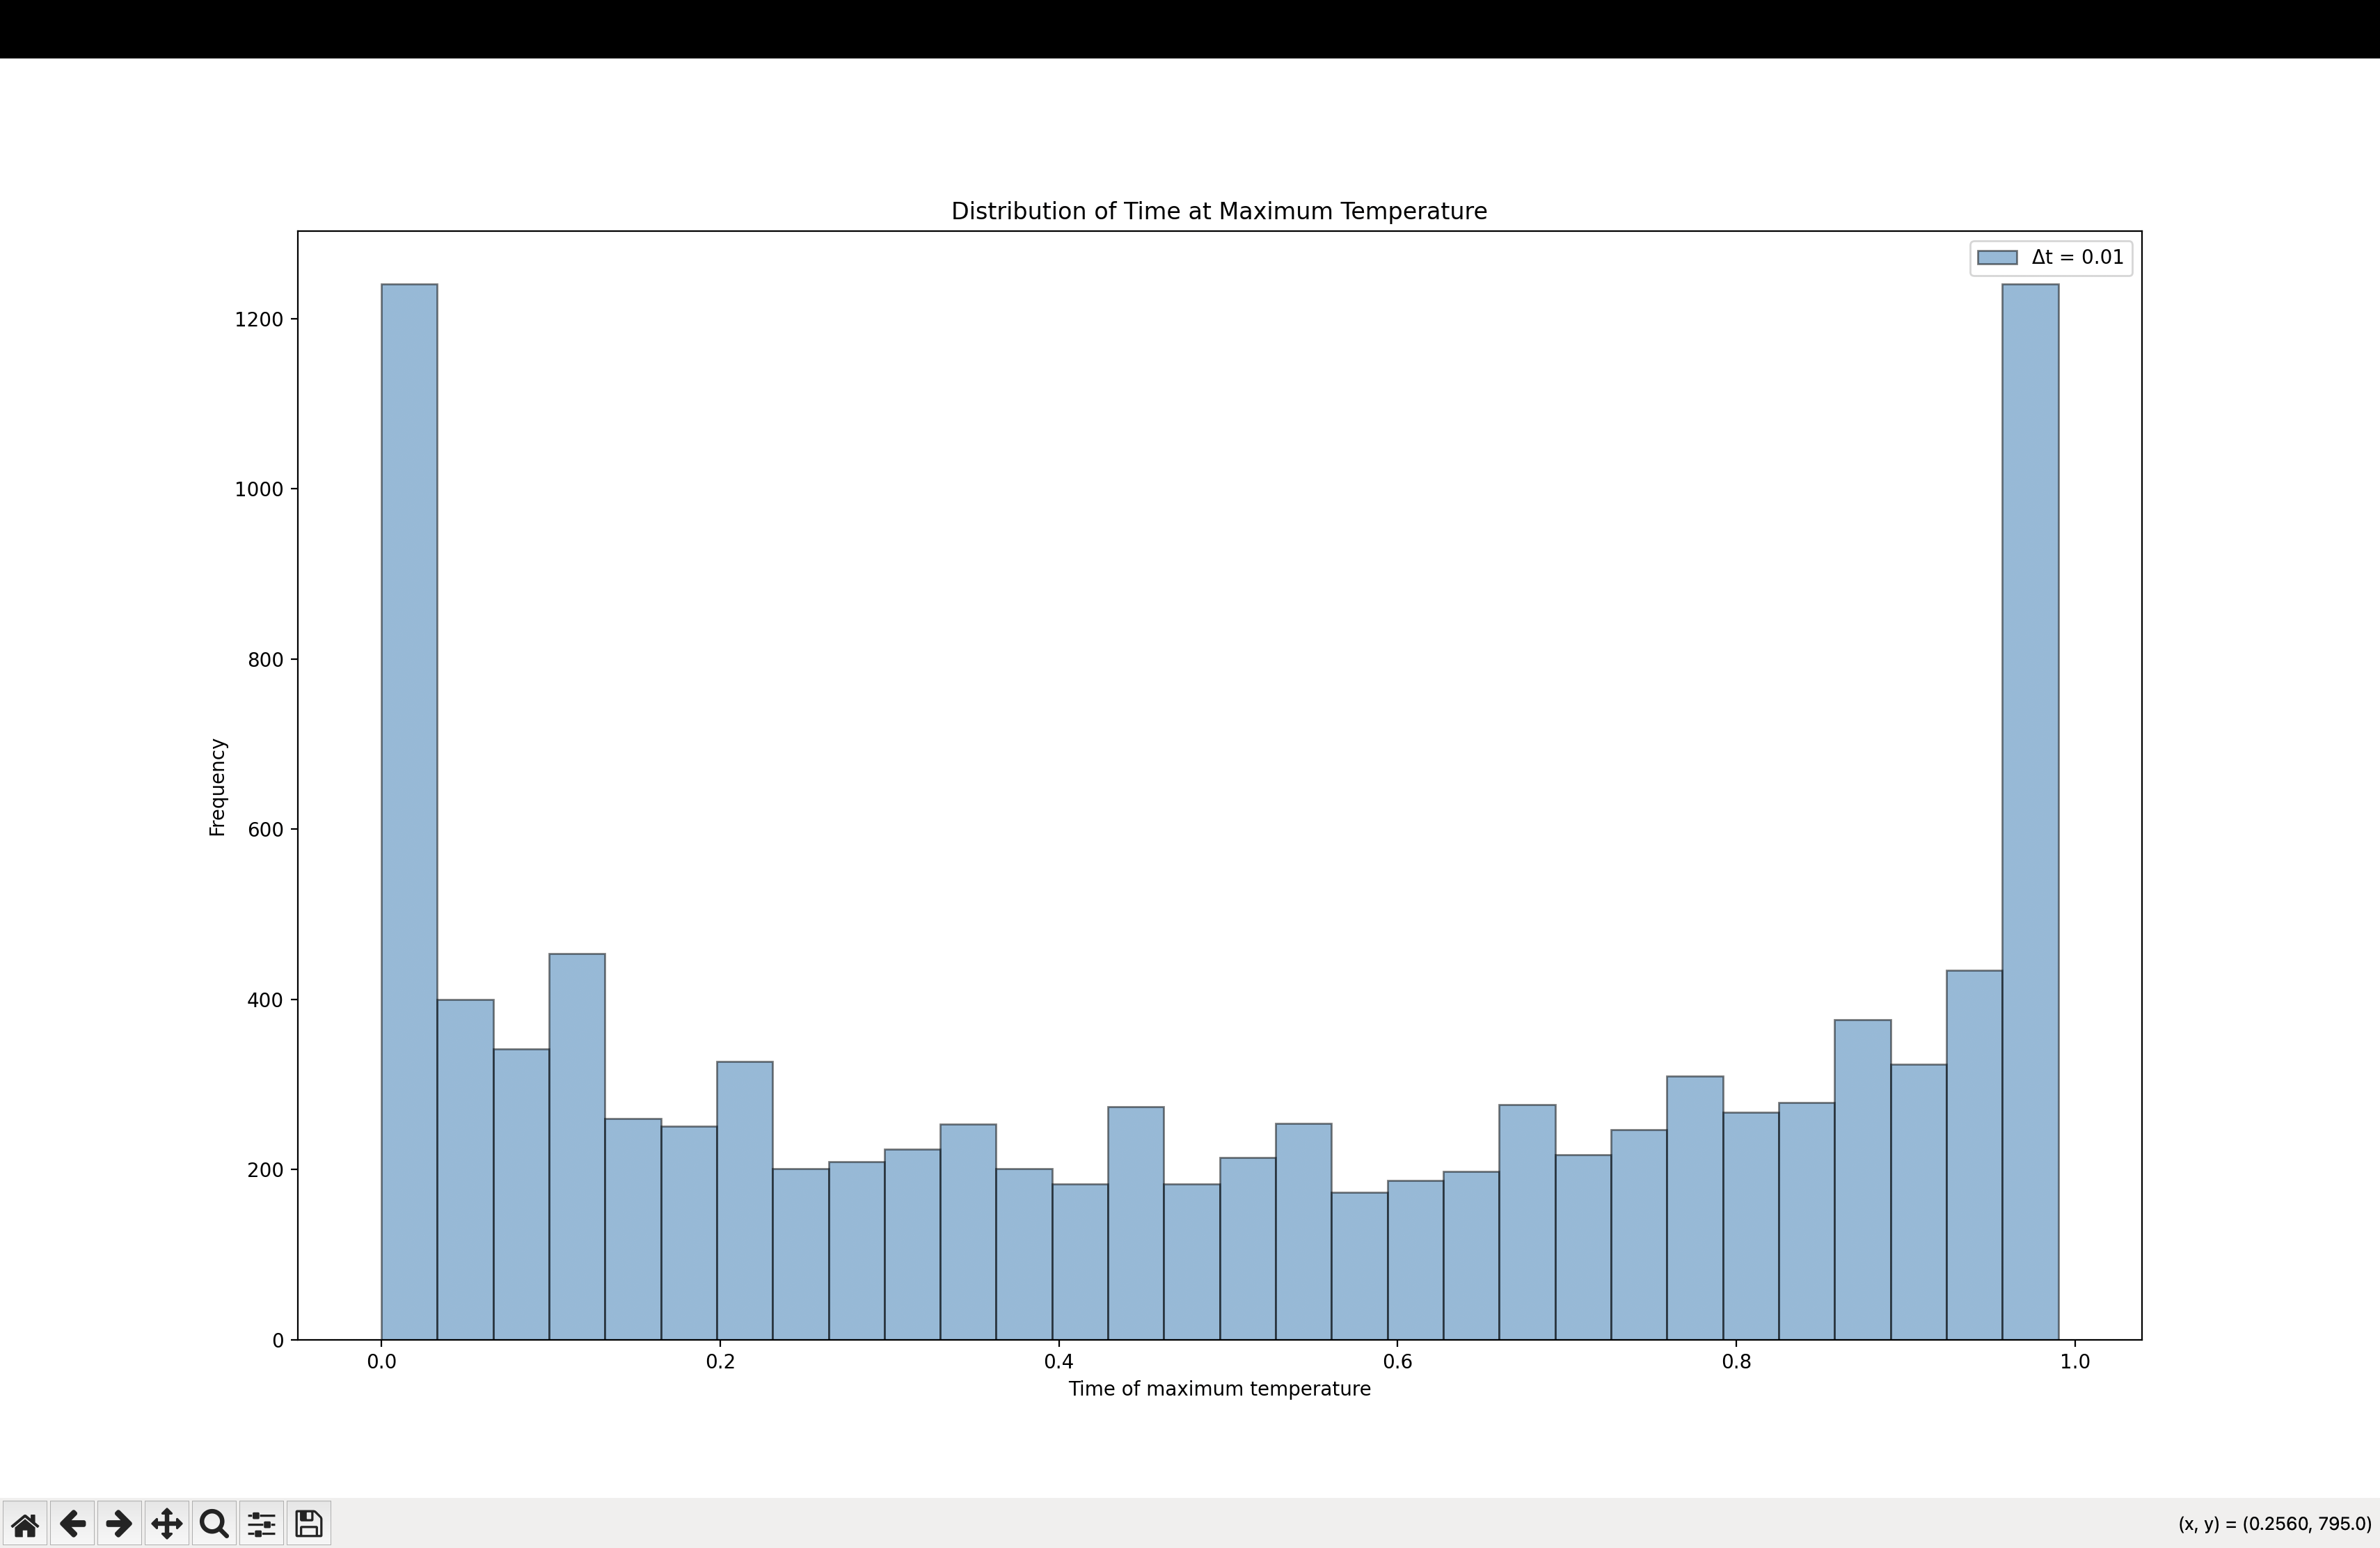
\includegraphics[width=0.6\textwidth]{q1_p2_f1.png}

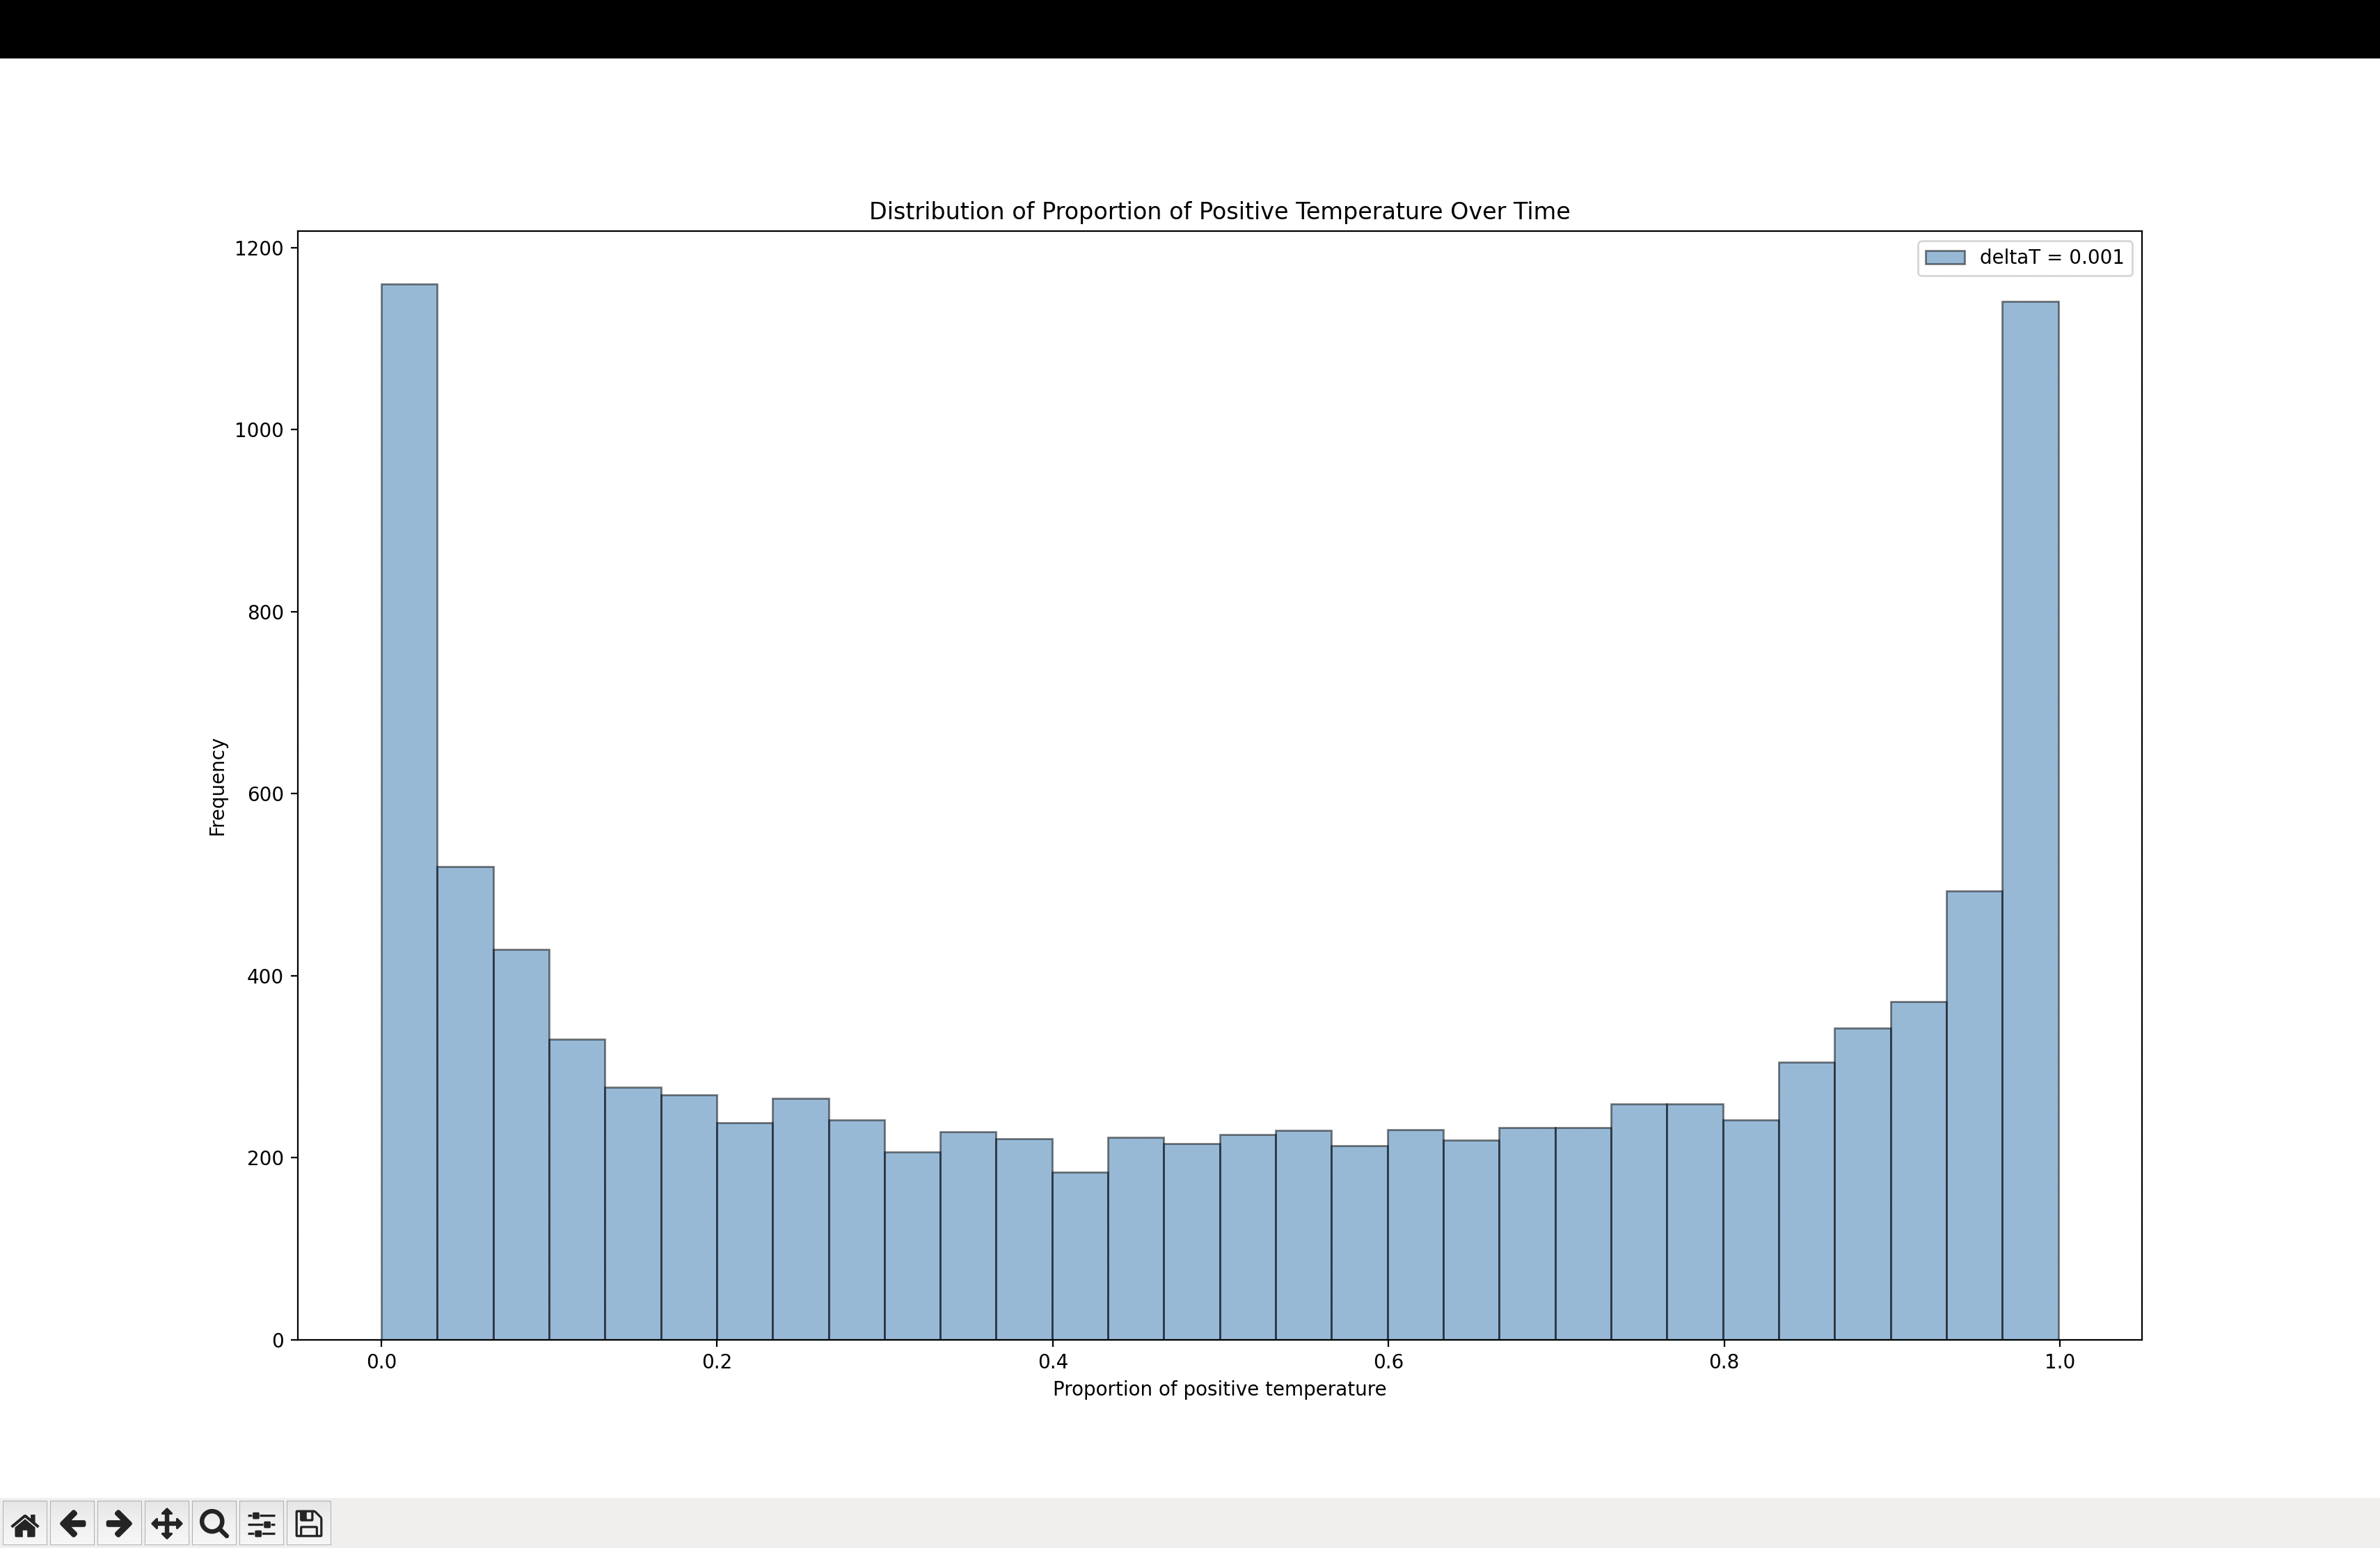
\includegraphics[width=0.6\textwidth]{q1_p1_f2.png}\\

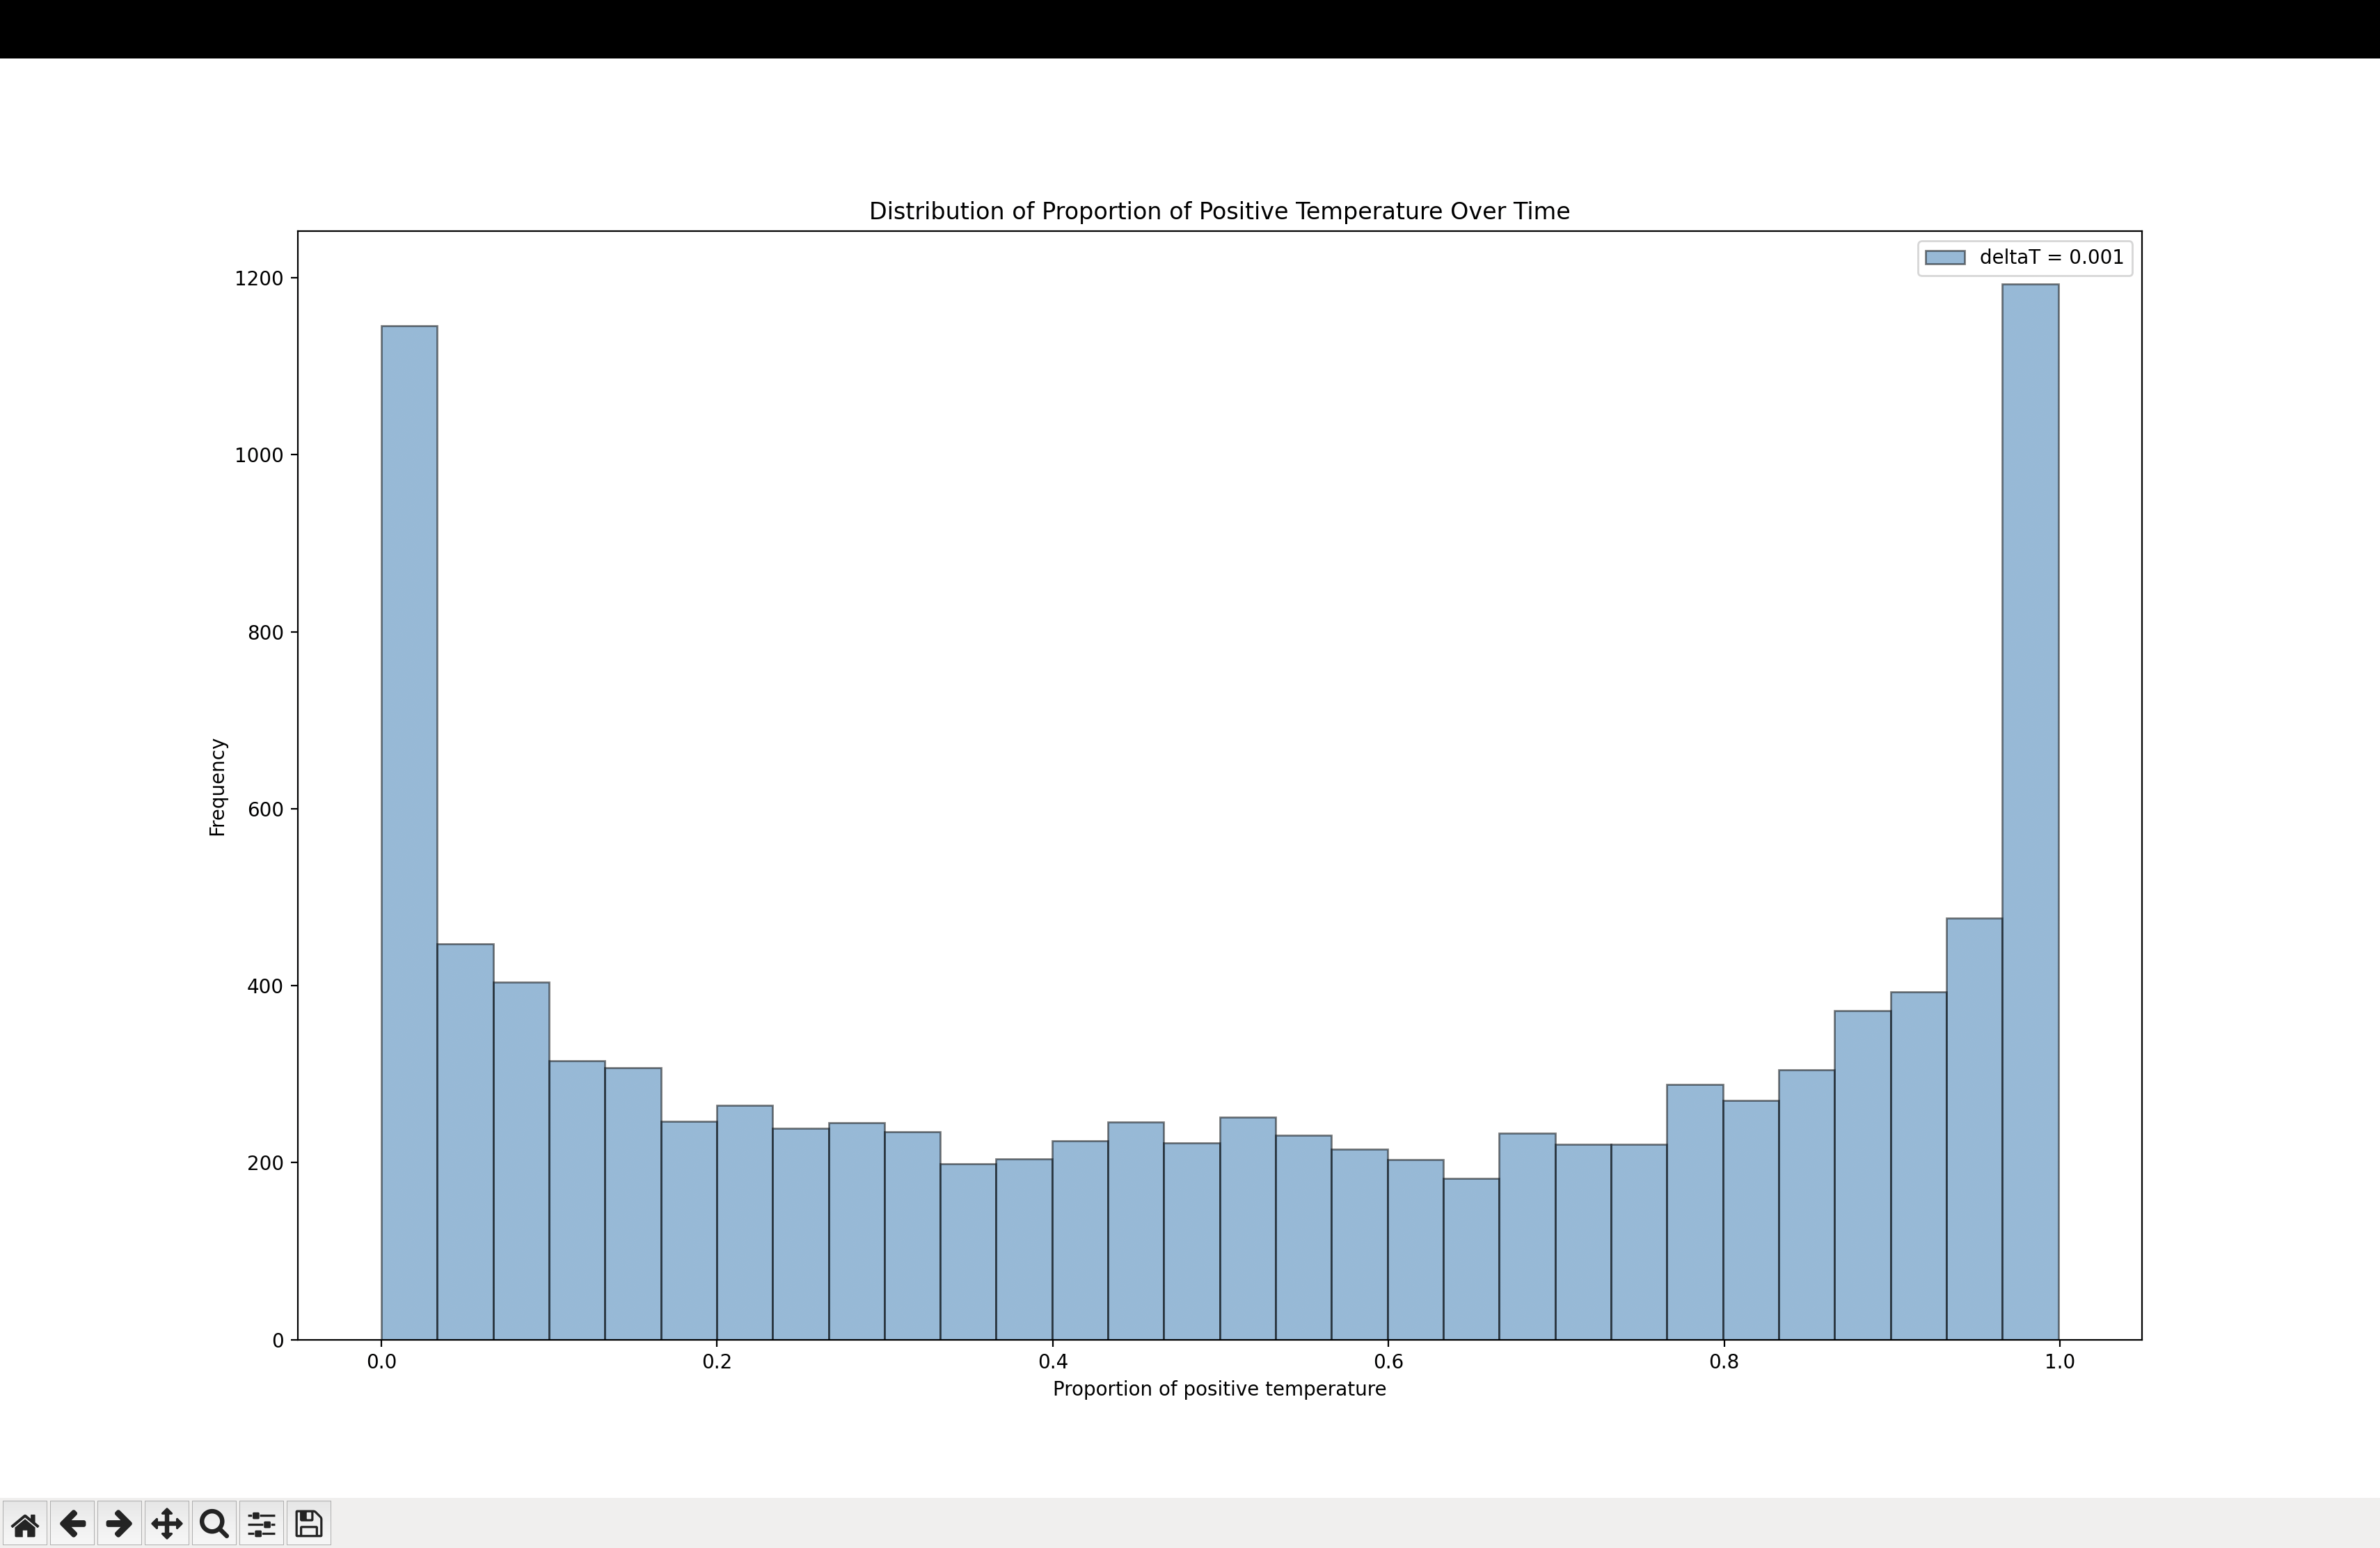
\includegraphics[width=0.6\textwidth]{q1_p1_f3.png}\\

\newpage
\section*{Question 2}
Create a probabilistic model and perform Monte Carlo simulations to forecast the final points for Premier League teams in the 2024-2025 season. This model will include some unknown parameters that you will determine based on the data you gather. In Premier League matches, teams earn three points for a win, one point for a draw, and no points for a loss. For your predictions, you could use statistics from the beginning of the season up to a specific date to estimate the parameters of your model, and then run Monte Carlo simulations to project the outcomes of the remaining matches, ultimately predicting the final points for each team at the season's end.\\

Here's a brief outline of a relatively straightforward way to model this scenario. For each match, you can treat the number of shots attempted by the home and away teams as random variables, such as Poisson random variables. The rate parameters of the Poisson distribution will be influenced by the strengths of both teams. Each shot taken will have an associated probability of scoring, which also varies depending on the teams involved.\\

You are encouraged to create your own models, but it's essential to explain and justify your choices. Discuss how you determine the parameters and outline the advantages and limitations of the models you select.\\

You can collect data from various online sources, such as this example: \url{https://www.premierleague.com/stats/top/clubs/total_scoring_att}.

\subsection*{Method}

\lipsum[1]\\

\lipsum[2]\\

\lipsum[3]\\

\lipsum[4]\\

\lipsum[5]

\subsection*{Code}

\subsubsection*{Version 1}

\begin{verbatim}
    import pandas as pd
    import numpy as np
    
    # Load league table and fixtures data
    league_table_df = pd.read_csv('/Users/lauri/Documents/College/STU22004-202425 
    ST2004 APPLIED PROBABILITY I/LeagueTable-Table1.csv')
    fixtures_df = pd.read_csv('/Users/lauri/Documents/College/STU22004-202425 ST2004 
    APPLIED PROBABILITY I/fixtures-Table 1.csv')
    
    # Filter league table relevant columns
    league_table_df_filtered = league_table_df[['Team', 'MP', 'GF', 'GA', 
    'Points']].dropna()
    
    # Calculate average goals scored (GF) and conceded (GA) per match
    league_table_df_filtered['Avg_GF_per_match'] = league_table_df_filtered['GF'] / 
    league_table_df_filtered['MP']
    league_table_df_filtered['Avg_GA_per_match'] = league_table_df_filtered['GA'] / 
    league_table_df_filtered['MP']
    
    # Prepare fixtures for simulation
    fixtures_df_filtered = fixtures_df[['Match Day', 'Home Team', 'Away Team', 
    'Likely Home Goal', 'Likely Away Goal']].dropna()
    
    # Monte Carlo simulation parameters
    num_simulations = 1000
    remaining_matches = fixtures_df_filtered.shape[0]
    
    # Initialize a dictionary to hold final point forecasts for each team across 
    simulations
    team_final_points = {team: [] for team in league_table_df_filtered['Team']}
    
    # Run Monte Carlo simulations
    for _ in range(num_simulations):
        # Initialize a dictionary to hold points for this simulation run
        points_simulation = league_table_df_filtered.set_index('Team')['Points'].
        to_dict()
    
        # Simulate remaining matches
        for _, row in fixtures_df_filtered.iterrows():
            home_team = row['Home Team']
            away_team = row['Away Team']
            home_goal_avg = row['Likely Home Goal']
            away_goal_avg = row['Likely Away Goal']
    
            # Simulate goals using Poisson distribution
            home_goals = np.random.poisson(home_goal_avg)
            away_goals = np.random.poisson(away_goal_avg)
    
            # Assign points based on match outcome
            if home_goals > away_goals:
                points_simulation[home_team] += 3
            elif home_goals < away_goals:
                points_simulation[away_team] += 3
            else:
                points_simulation[home_team] += 1
                points_simulation[away_team] += 1
    
        # Store the points from this simulation run
        for team in team_final_points:
            team_final_points[team].append(points_simulation.get(team, 0))
    
    # Compute average final points per team after simulations
    forecasted_points = {team: np.mean(points) for team, points in team_final_points
    .items()}
    forecasted_points_df = pd.DataFrame(list(forecasted_points.items()), columns=
    ['Team', 'Forecasted Points']).sort_values(by='Forecasted Points', ascending=False)
    
    # Display forecasted final points
    print("Forecasted Final Points for Premier League Teams")
    print(forecasted_points_df)
\end{verbatim}

\subsubsection*{Version 2}

\begin{verbatim}
    import pandas as pd
    import numpy as np
    from tqdm import tqdm  # Import tqdm for the progress bar

    # Load league table and fixtures data
    league_table_df = pd.read_csv('q2_pdfs/LeagueTable.csv')
    fixtures_df = pd.read_csv('q2_pdfs/FixtureTable.csv')

    # Filter relevant columns from the league table
    league_table_df_filtered = league_table_df[['Team', 'MP', 'GF', 'GA', 'Points', 
    'Poss', 'CrdY', 'CrdR']].dropna()

    # Calculate average goals scored (GF) and conceded (GA) per match
    league_table_df_filtered['Avg_GF_per_match'] = league_table_df_filtered['GF'] / 
    league_table_df_filtered['MP']
    league_table_df_filtered['Avg_GA_per_match'] = league_table_df_filtered['GA'] / 
    league_table_df_filtered['MP']

    # Prepare fixtures for simulation
    fixtures_df_filtered = fixtures_df[['Match Day', 'Home Team', 'Away Team', 
    'Likely Home Goal', 'Likely Away Goal']].dropna()

    # Monte Carlo simulation parameters
    num_simulations = 1000

    # Initialize a dictionary to hold final point forecasts for each team across 
    simulations
    team_final_points = {team: [] for team in league_table_df_filtered['Team']}

    # Helper function to adjust goal averages
    def adjust_goals(base_goals, possession, yellow_cards, red_cards):
        possession_factor = 1 + (possession - 50) / 100  # Scale possession effect
        discipline_factor = max(0.9, 1 - (0.05 * yellow_cards + 0.1 * red_cards))  
        # Penalize for cards
        return base_goals * possession_factor * discipline_factor

    # Run Monte Carlo simulations with a progress bar
    for _ in tqdm(range(num_simulations), desc="Simulating Matches", 
    unit="simulation"):
        # Initialize a dictionary to hold points for this simulation run
        points_simulation = league_table_df_filtered.set_index('Team')
        ['Points'].to_dict()

        # Simulate remaining matches
        for _, row in fixtures_df_filtered.iterrows():
            home_team = row['Home Team']
            away_team = row['Away Team']
            home_goal_avg = row['Likely Home Goal']
            away_goal_avg = row['Likely Away Goal']
            
            # Retrieve possession and card metrics for both teams
            home_stats = league_table_df_filtered[league_table_df_filtered['Team'] 
            == home_team].iloc[0]
            away_stats = league_table_df_filtered[league_table_df_filtered['Team'] 
            == away_team].iloc[0]

            home_possession = home_stats['Poss']
            home_yellow_cards = home_stats['CrdY']
            home_red_cards = home_stats['CrdR']

            away_possession = away_stats['Poss']
            away_yellow_cards = away_stats['CrdY']
            away_red_cards = away_stats['CrdR']

            # Adjust goals based on possession and discipline factors
            home_goal_avg = adjust_goals(home_goal_avg, home_possession, 
            home_yellow_cards, home_red_cards)
            away_goal_avg = adjust_goals(away_goal_avg, away_possession, 
            away_yellow_cards, away_red_cards)

            # Simulate goals using Poisson distribution
            home_goals = np.random.poisson(home_goal_avg)
            away_goals = np.random.poisson(away_goal_avg)

            # Assign points based on match outcome
            if home_goals > away_goals:
                points_simulation[home_team] += 3
            elif home_goals < away_goals:
                points_simulation[away_team] += 3
            else:
                points_simulation[home_team] += 1
                points_simulation[away_team] += 1

        # Store the points from this simulation run
        for team in team_final_points:
            team_final_points[team].append(points_simulation.get(team, 0))

    # Compute average final points per team after simulations
    forecasted_points = {team: np.mean(points) for team, points in 
    team_final_points.items()}
    forecasted_points_df = pd.DataFrame(list(forecasted_points.items()), 
    columns=['Team', 'Forecasted Points']).sort_values(by='Forecasted Points', 
    ascending=False)

    # Display forecasted final points
    print("Forecasted Final Points for Premier League Teams")
    print(forecasted_points_df)
\end{verbatim}

\subsection*{Tables}

See next page

\begin{table}[p]
    \centering
    \begin{tabular}{rlr}
    \toprule
    \textbf{Rank} & \textbf{Team} & \textbf{Forecasted Points} \\
    \midrule
    1  & Man City         & 113.241 \\
    2  & Liverpool        & 100.449 \\
    3  & Newcastle        & 92.759  \\
    4  & Arsenal          & 92.397  \\
    5  & Brighton         & 88.707  \\
    6  & Man Utd          & 80.455  \\
    7  & Aston Villa      & 78.171  \\
    8  & Chelsea          & 77.504  \\
    9  & Brentford        & 75.874  \\
    10 & Spurs            & 65.533  \\
    11 & Fulham           & 64.046  \\
    12 & West Ham         & 62.117  \\
    13 & Crystal Palace   & 60.677  \\
    14 & Leicester City   & 52.262  \\
    15 & Everton          & 51.254  \\
    16 & Nott'm Forest    & 48.809  \\
    17 & Bournemouth      & 47.729  \\
    18 & Ipswich Town     & 33.695  \\
    19 & Wolves           & 33.385  \\
    20 & Southampton      & 32.417  \\
    \bottomrule
    \end{tabular}
    \caption{Forecasted Final Points for Premier League Teams (Version 1)}
    \label{tab:forecasted_points_2}
    \vspace{1cm}
\end{table}

\vspace{1cm}

\begin{table}[p]
    \centering
    \begin{tabular}{rlr}
    \toprule
    \textbf{Rank} & \textbf{Team} & \textbf{Forecasted Points} \\
    \midrule
    1  & Man City         & 114.740 \\
    2  & Liverpool        & 101.445 \\
    3  & Arsenal          & 91.282  \\
    4  & Newcastle        & 90.681  \\
    5  & Brighton         & 88.536  \\
    6  & Man Utd          & 79.442  \\
    7  & Chelsea          & 78.706  \\
    8  & Aston Villa      & 78.212  \\
    9  & Brentford        & 73.697  \\
    10 & Spurs            & 68.335  \\
    11 & Fulham           & 64.667  \\
    12 & West Ham         & 60.992  \\
    13 & Crystal Palace   & 58.614  \\
    14 & Leicester City   & 51.757  \\
    15 & Everton          & 48.796  \\
    16 & Nott'm Forest    & 47.854  \\
    17 & Bournemouth      & 47.509  \\
    18 & Southampton      & 34.431  \\
    19 & Wolves           & 33.130  \\
    20 & Ipswich Town     & 32.519  \\
    \bottomrule
    \end{tabular}
    \caption{Forecasted Final Points for Premier League Teams (Version 2)}
    \label{tab:forecasted_points}
\end{table}

\end{document}